\section{Systembeskrivelse}
På Ingeniørhøjskolen Aarhus Universitet forefindes en AeroQuad ARF Quadrocopter. 
Målet med projektet er at omdanne quadrocopteren til en autonom overvågningsdrone.

Dronen skal ud fra brugers anvisninger overvåge og tage billeder af et defineret område. Webapplikation fungerer som et grafisk brugerflade mellem bruger og server.  
Via webapplikationen skal bruge kunne oprette flyveopsætninger til dronen samt se billeder og flyverute fra tidligere flyvninger. 
Når der laves ny flyveopsætning vælger bruger en række GPS positioner som dronen skal flyve til, flyvehøjde og hvorvidt der skal tages billeder ved de valgte GPS positioner. Når bruger har lavet en ny flyveopsætning, stilles flyveopsætningen tilgængelig for dronen på server.  

Til enhver tid, skal al kommunikation mellem drone og server foregå via mobil netværk. Der gøres hovedsageligt brug af 3G netværket, men i områder med dårlig forbindelse vil der blive gjort brug af 2G som fall-back netværk. Da dronen skal flyve autonomt, er det vigtigt den kan orientere sig på egen hånd. Derfor er den udstyres den med GPS, afstands sensorer og kompas.



\section{Systemoversigt}
Nederst til højre på figur \ref{fig:Systemskitse} ses et device. Dette device benyttes af bruger til at tilgå webapplikation, og lave en ny flyveopsætning. Når bruger har lavet en ny flyveopsætning, overføres flyveopsætningen via internettet til server, hvor den gøres tilgængelig for dronen.
 
Under flyvning kontrollerer dronen løbende egen GPS position via kommunikation med GPS satellitter. Dette gør dronen for at opdatere egen position og for efterfølgende at kunne beregne den korrekte flyveorientering. 
Via det mobile 3G netværk kommunikerer drone løbende med server. Dronen fortæller server om nuværende GPS position, overføre billeder og tjekker om der er nye flyveopsætninger tilgængelig. 

\vspace{-5pt}
%Systemskitse
\begin{figure}[H]
\centering
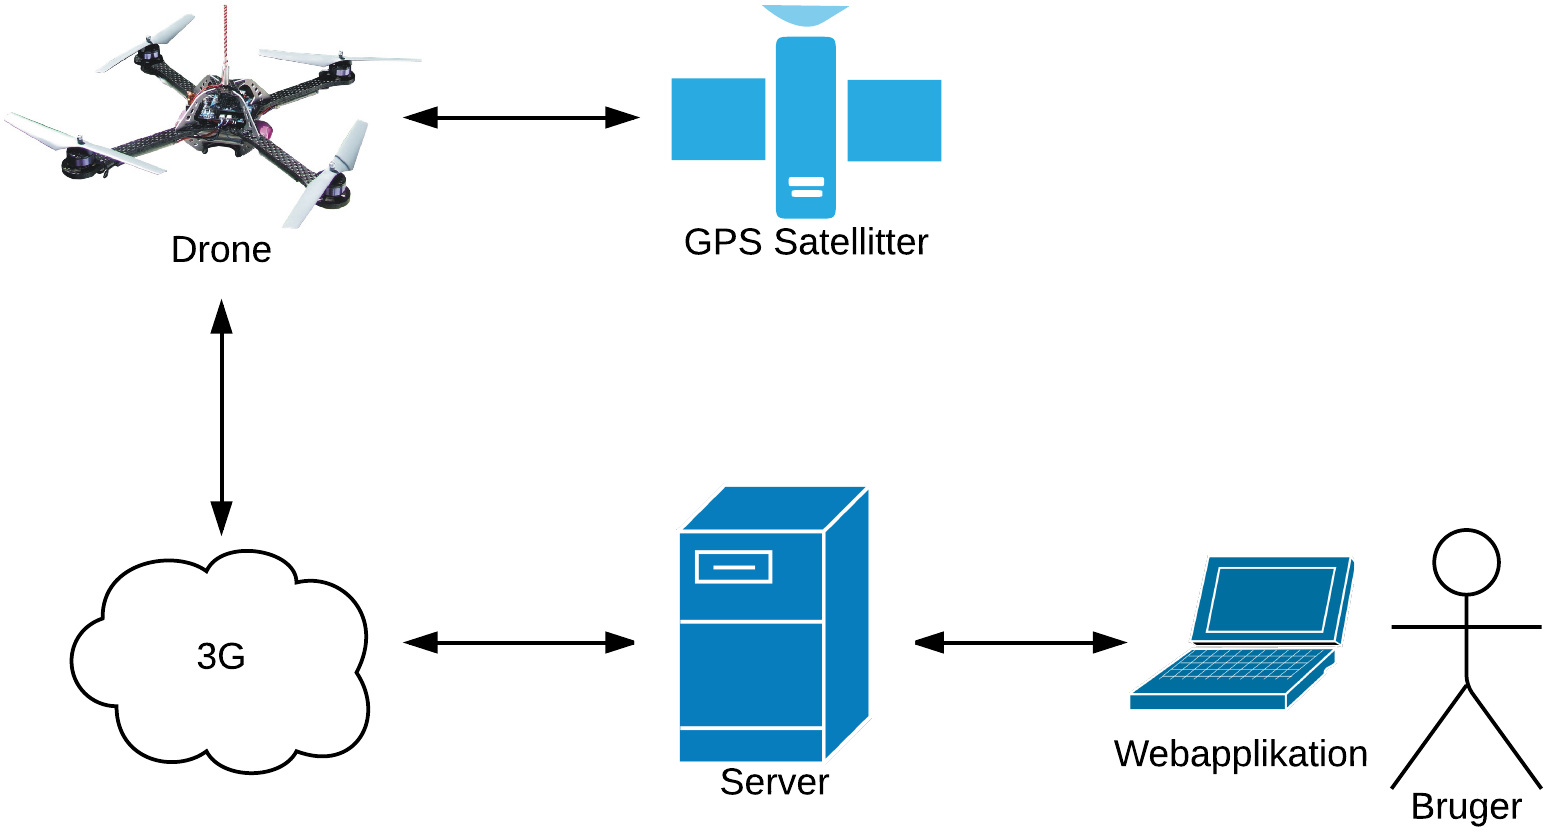
\includegraphics[width=1\textwidth]{Billeder/Projektbeskrivelse.png}
\vspace{-.5cm}
\caption{Systemskitse}
\label{fig:Systemskitse}
\end{figure}